This chapter compares a suite of weak lensing statistics derived from two sets of simulations: BIGBOX and TILED. Our goal is to quantify differences in mean values, covariance, and correlation matrices to assess how super-sample covariance and other systematic effects influence these measurements. We will also examine how shape noise, smoothing scales, and box replication artifacts affect the results.

\section{Comparison of Mean and Variance for Statistical Measures}
We compare the mean values $\mu$ and variances $\sigma^2$ of statistical measures derived from the BIGBOX and TILED simulations. 
Figures~\ref{fig:ell_main} and~\ref{fig:nu_main} present the comparisons of both mean and variance for the angular power spectrum, bispectrum, and other higher-order statistics.

The mean values are generally consistent between the two simulations, with differences below $1\%$ in the ratio $R_{\mu}$ for most statistics. However, common deviations are observed at low $\nu$ values for peak counts, minima, and Minkowski Functionals. These deviations indicate limitations in the TILED simulations to resolve low-density regions. 

Variance ratios $R_{\sigma^2}$ highlight the impact of super-sample covariance, particularly evident in the diagonal elements of the covariance matrices. As expected, the angular power spectrum in the BIGBOX simulations demonstrates increased power at high $\ell$ values due to super-sample effects. Moreover, the discrepancy between the BIGBOX and TILED simulations increases with source redshift, as the TILED simulations lose more large-scale modes.

All $\nu$-binned statistics display higher variances in the BIGBOX simulations across nearly all $\nu$ bins, and the ratios of variances increase with source redshift. This trend suggests the presence of super-sample covariance in these statistical measures, underscoring its significant influence on the covariance structures.

\begin{figure}[ht]
    \centering
    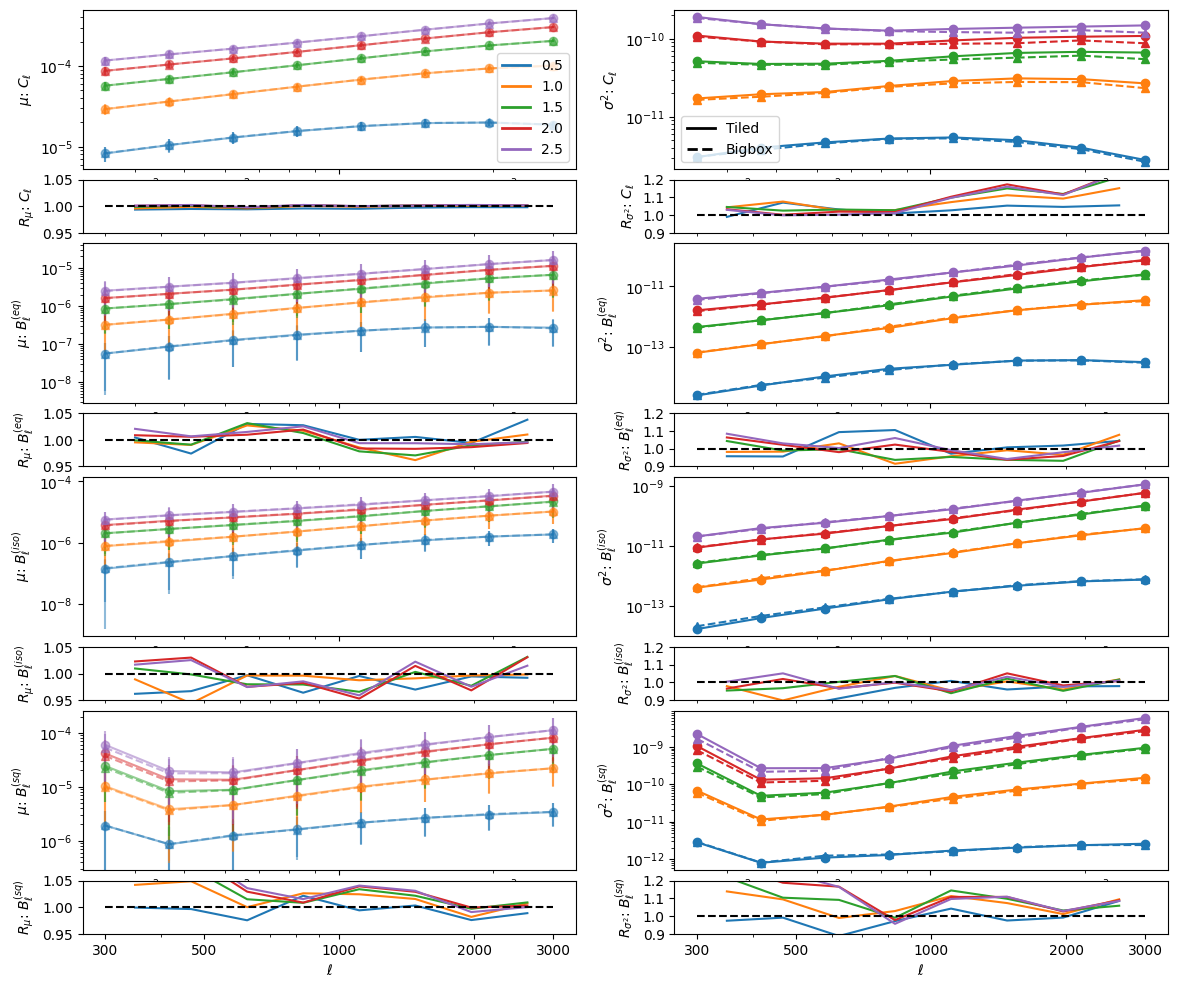
\includegraphics[width=\textwidth]{figures/results/ell_main.png}
    \caption[Comparison of the mean and variance of $C^{\kappa\kappa}_{\ell}$ and Bispectrum]{Comparison of the mean and variance of the angular power spectrum ($C^{\kappa\kappa}_{\ell}$) and bispectrum of three configurations ($B_{\ell}^{(eq)}, B_{\ell}^{(iso)}, B_{\ell}^{(sq)}$) between the BIGBOX and TILED simulations for multiple source redshifts ($z_s = 0.5, 1.0, 1.5, 2.0, 2.5$).}
    \label{fig:ell_main}
\end{figure}

\begin{figure}[p]
    \centering
    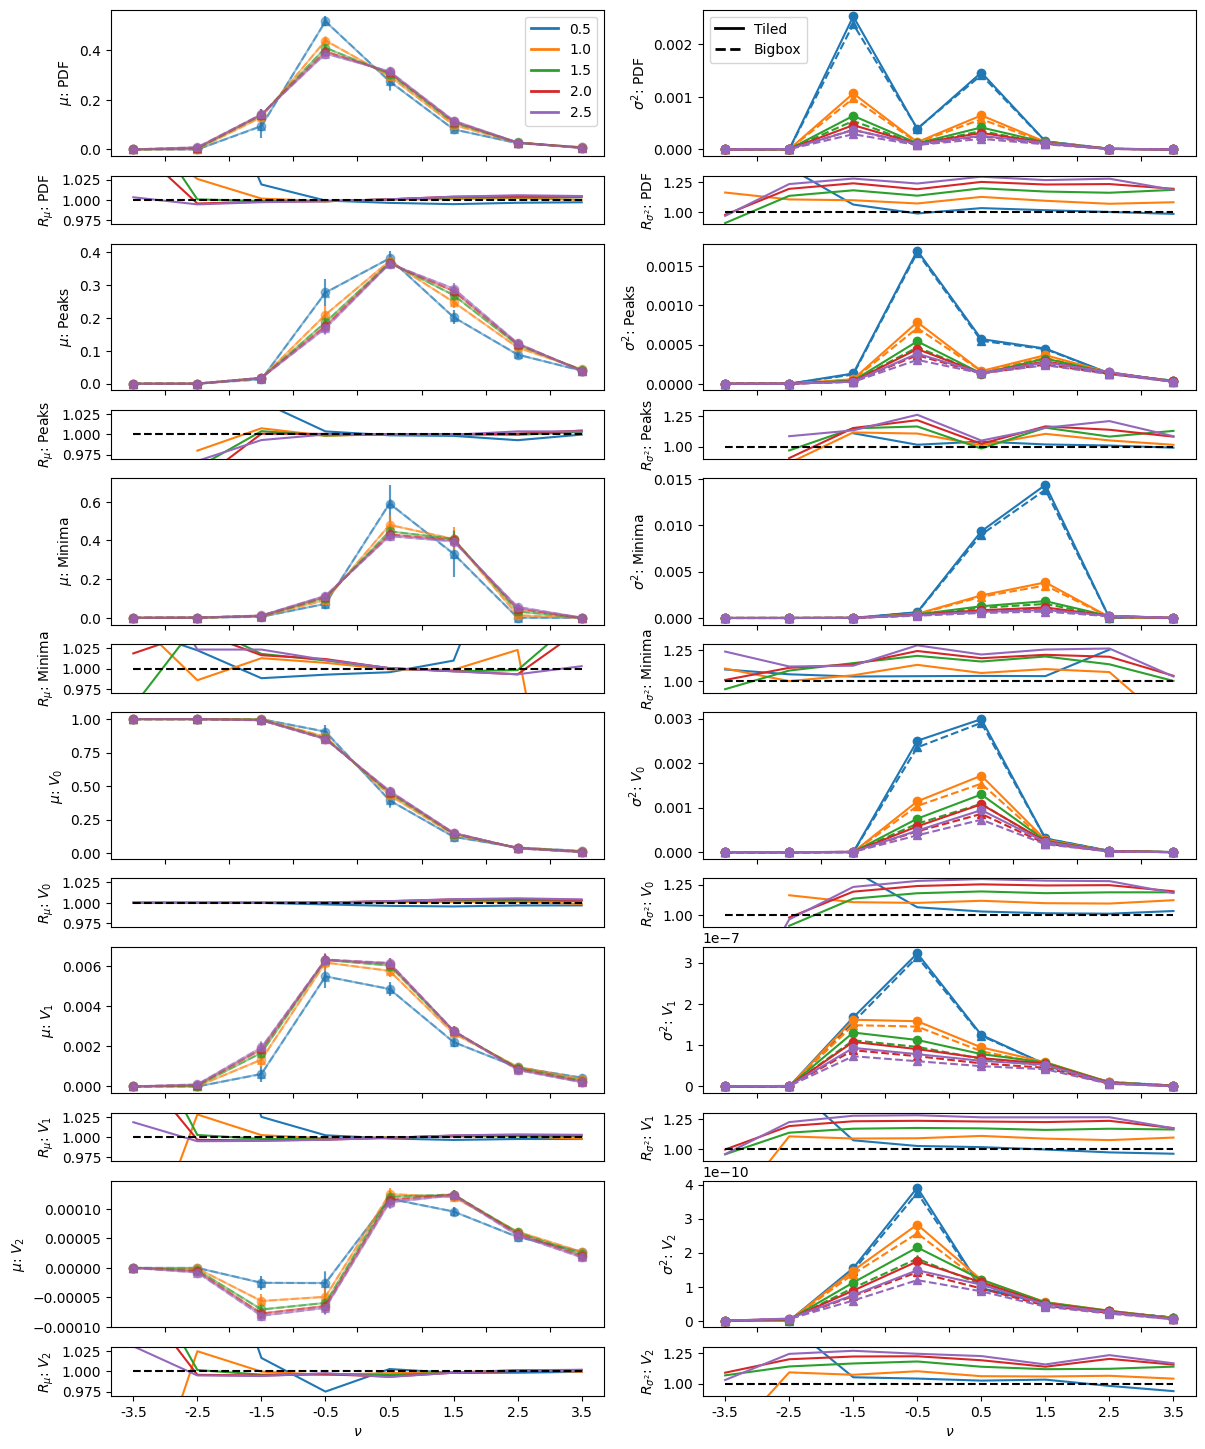
\includegraphics[width=\textwidth]{figures/results/nu_main.png}
    \caption[Comparison of the mean and variance of Non-Correlation Statistics]{Comparison of the mean and variance of the probability density function (PDF), peak/minima counts, and Minkowski Functionals ($V_0, V_1, V_2$) between the BIGBOX and TILED simulations for multiple source redshifts ($z_s = 0.5, 1.0, 1.5, 2.0, 2.5$).}
    \label{fig:nu_main}
\end{figure}

\section{Analysis of Covariance and Correlation Matrices}
To quantify the super-sample covariance effects on off-diagonal terms, we also compare the covariance and correlation matrices of the statistical measures. Figures~\ref{fig:cov_main} and~\ref{fig:cov_ratio_main} give the covariance matrices $\text{Cov}_{ij}$ and their ratios $R^{\text{Cov}}_{ij}$ for each statistic at multiple source redshifts, while Figures~\ref{fig:corr_main} and~\ref{fig:corr_ratio_main} show the correlation matrices $\rho_{ij}$ and their ratios $R^{\rho}_{ij}$.

The figure indicate that $R_{\text{Cov}}$, the ratios of covariance matrix elements between the BIGBOX and TILED simulations, are consistently $10\%$ to $30\%$ higher than unity for most statistics.
This indicates that the BIGBOX simulations yield the same trend as in the diagonal terms, with higher covariance values compared to the TILED simulations. Moreover, the discrepancy between the BIGBOX and TILED simulations increases with source redshift. They supports the hypothesis that super-sample covariance significantly impacts the covariance structures of these statistics. 

$R_{\rho}$, the ratios of correlation matrix elements, indicate the presence of off-diagonal correlations in the angular power spectrum. For power spectrum, the correlation between small and large $\ell$ bins can be seen, which is consistent with the super-sample covariance effect. For PDF, peak counts, and Minkowski Functionals, the ratio are generally $ < 5\%$, indicating that the the super-sample effect is not only in the diagonal terms but also in the off-diagonal terms, lifting the overall covariance matrix.

\begin{figure}[p]
    \centering
    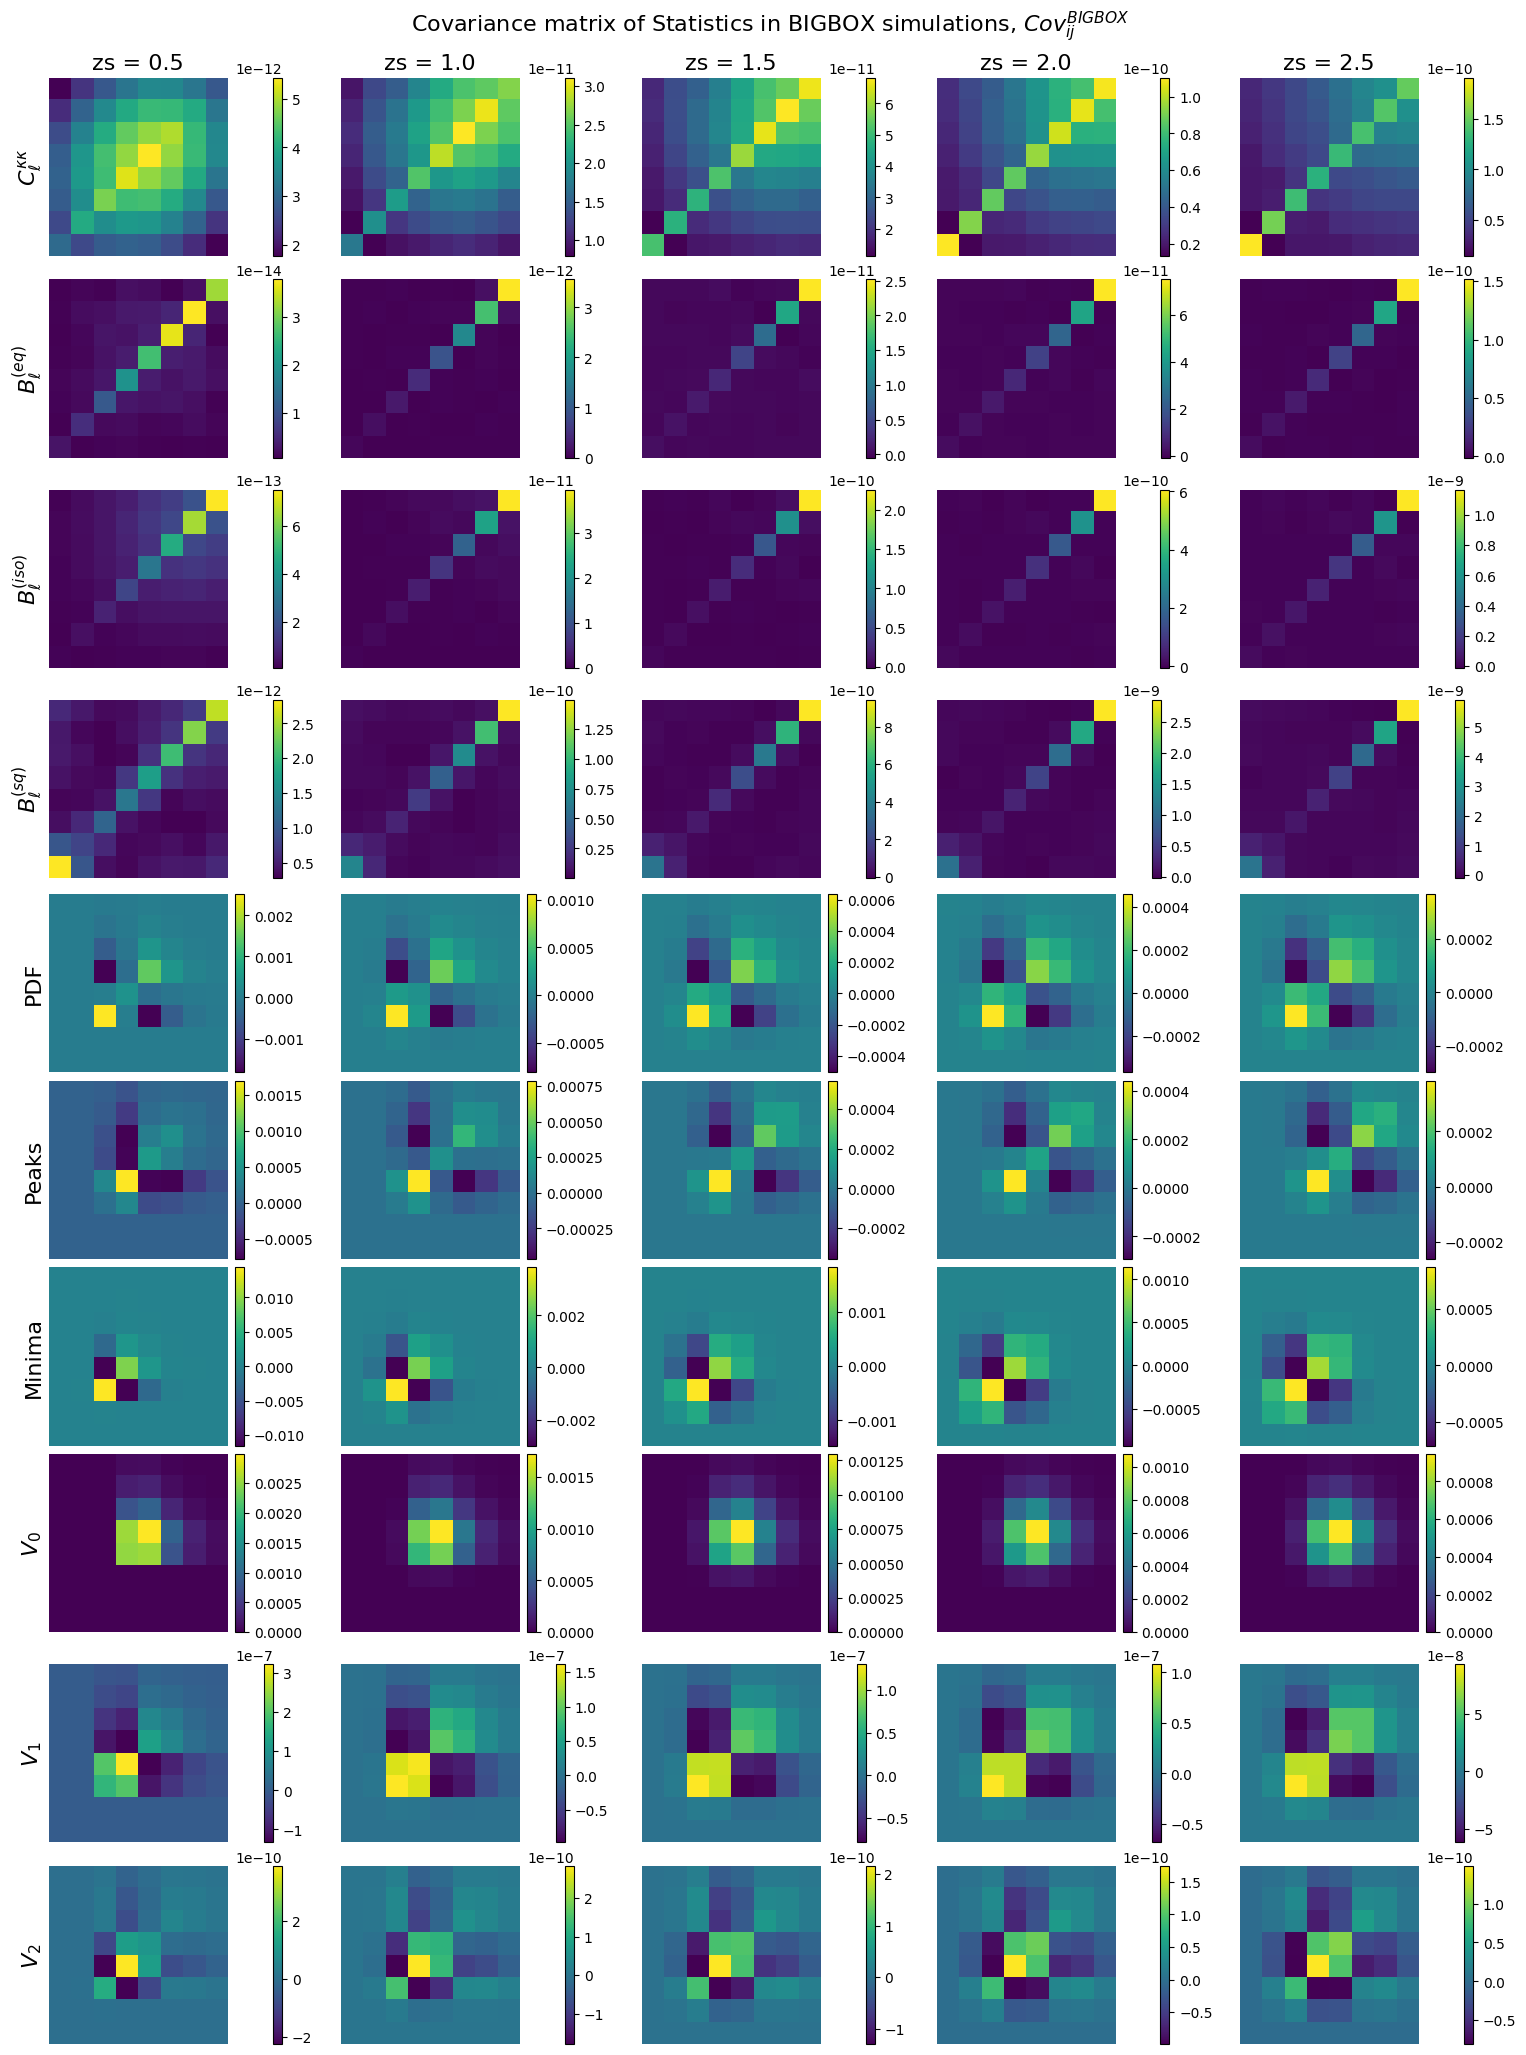
\includegraphics[width=\textwidth]{figures/results/cov_bigbox.png}
    \caption[Covariance Matrices of Statistical Measures in BIGBOX Simulations]{Covariance matrices of statistical measures in the BIGBOX simulations for multiple source redshifts ($z_s = 0.5, 1.0, 1.5, 2.0, 2.5$).}
    \label{fig:cov_bigbox}
\end{figure}

\begin{figure}[p]
    \centering
    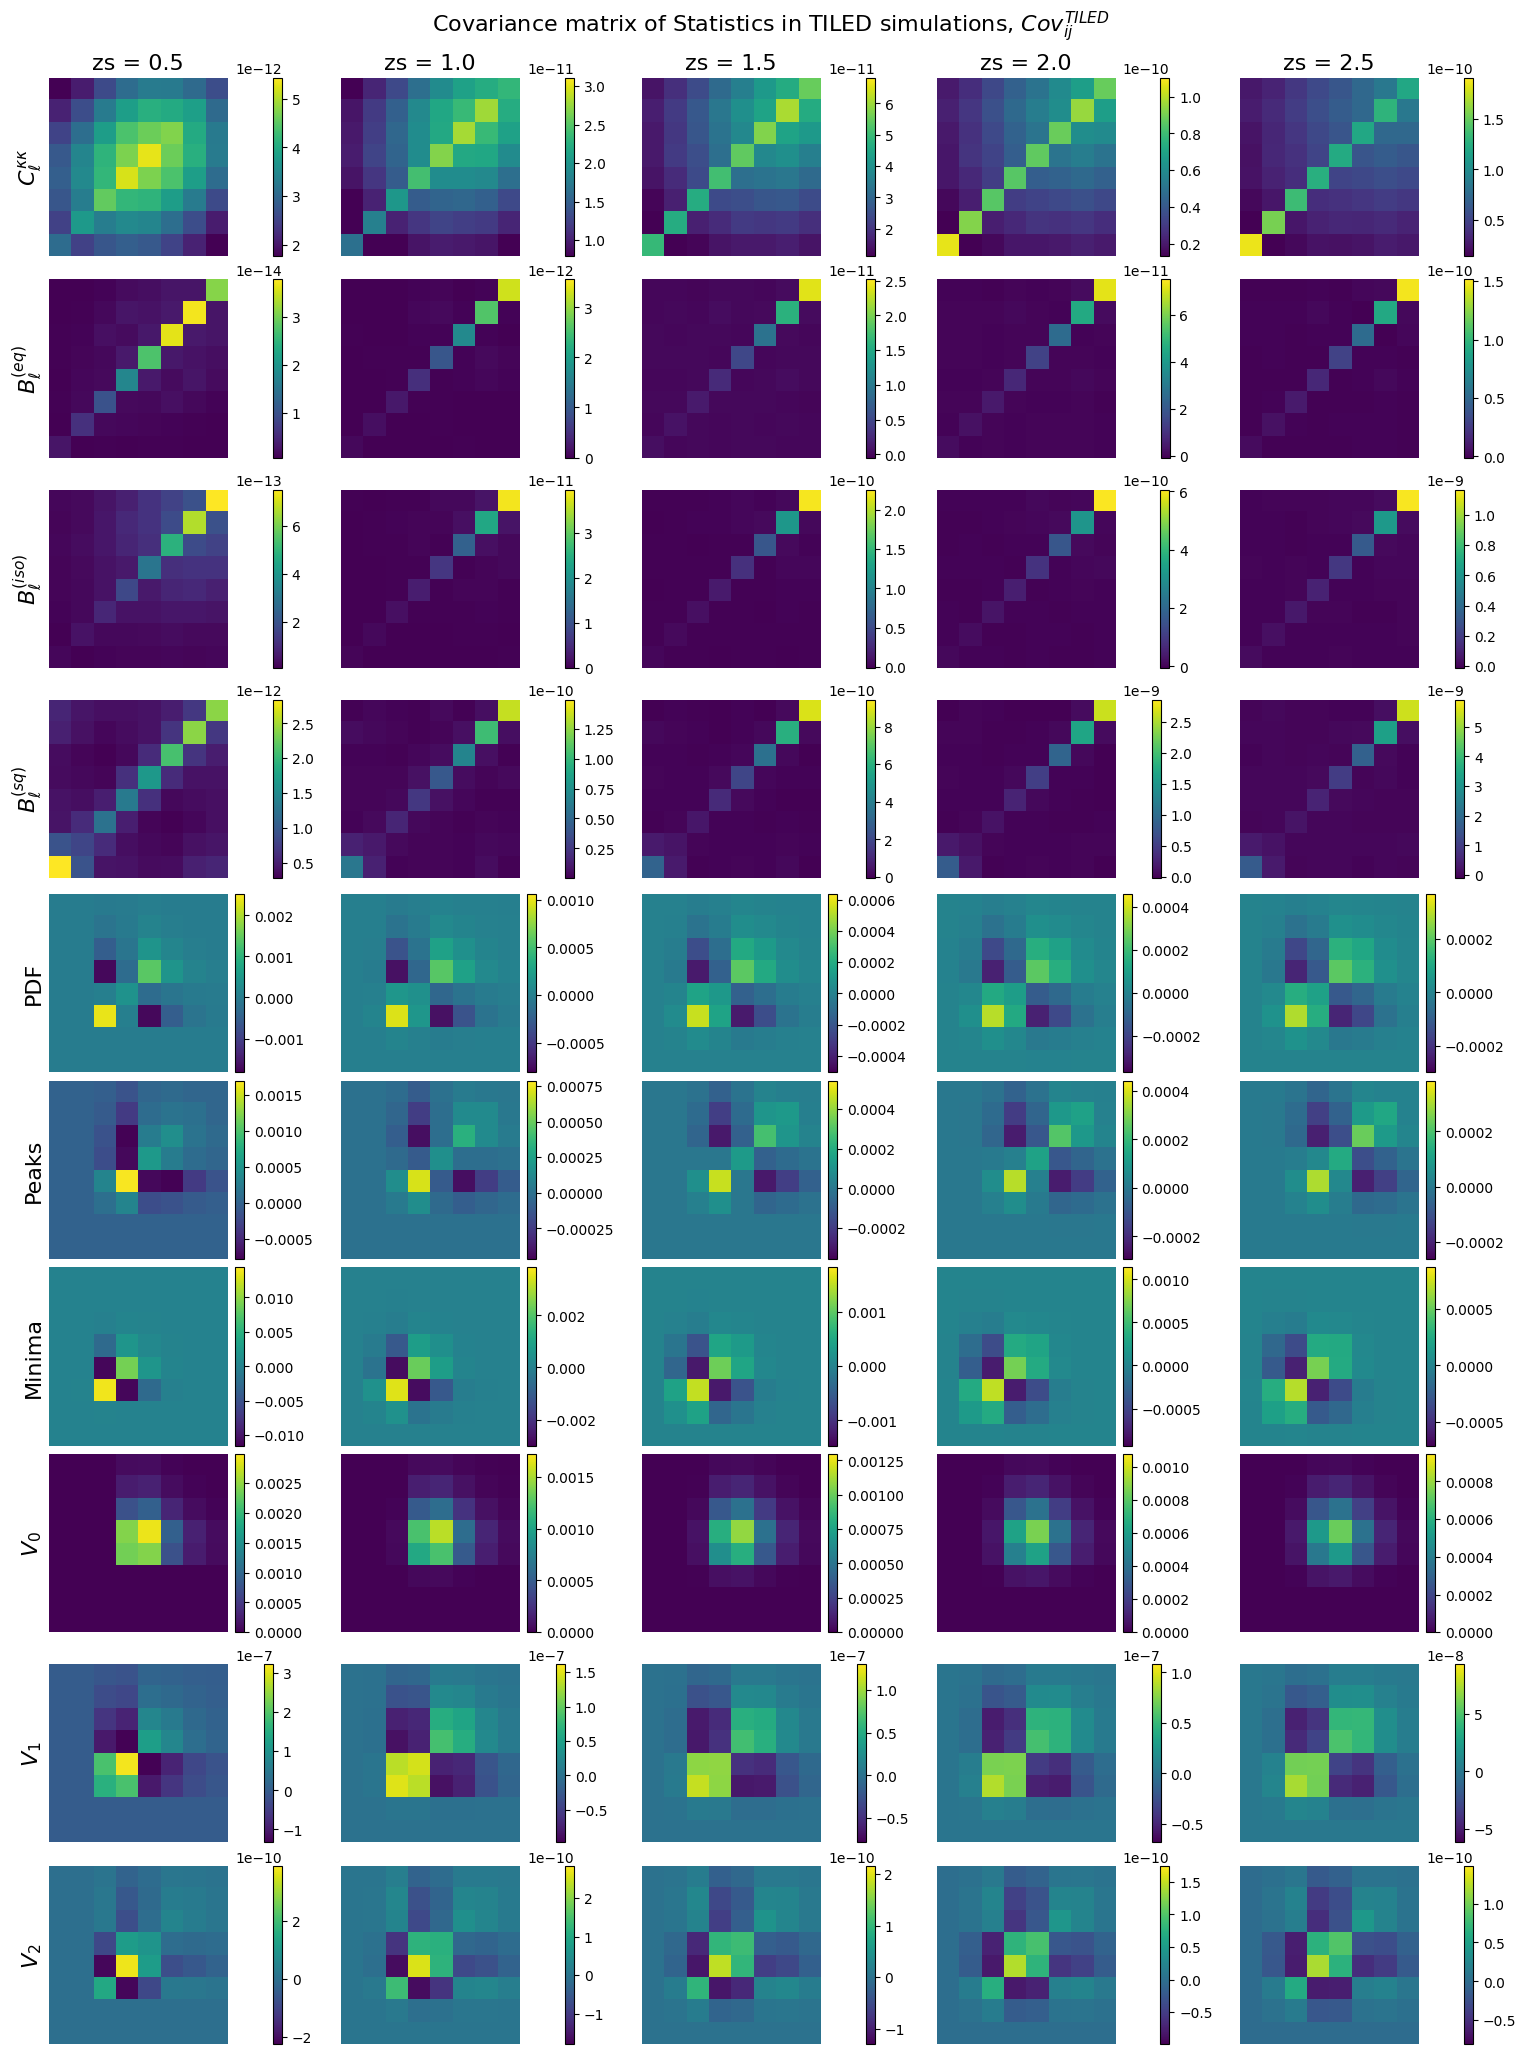
\includegraphics[width=\textwidth]{figures/results/cov_tiled.png}
    \caption[Covariance Matrices of Statistical Measures in TILED Simulations]{Covariance matrices of statistical measures in the TILED simulations for multiple source redshifts ($z_s = 0.5, 1.0, 1.5, 2.0, 2.5$).}
    \label{fig:cov_tiled}
\end{figure}

\section{Effects of Noise on Statistical Measures}
Introducing various levels of shape noise shows that while certain statistics, such as $C_\ell^{\kappa\kappa}$ and Minima Counts, are sensitive to noise-induced changes, other non-Gaussian measures remain relatively stable. This indicates that super-sample covariance could be commonly exist in the non-Gaussian statistics, and the noise level does not affect the covariance structures of these statistics.


\section{Influence of Smoothing Scale}
We investigate how applying different Gaussian smoothing scales alters the statistical measures. As smoothing increases, small-scale features are diminished and the distribution of signal intensities changes. Covariance ratios become more unstable as structures blur, underscoring that the choice of smoothing scale affects both the amplitude and the covariance patterns of measured statistics.

\section{Identifying and Addressing Systematic Effects}
\subsection{Box Replication Effect}
We isolate patches most affected by the repeated tiling of the simulation box and find that these regions introduce biases into mean values and inflations in covariance. Removing or carefully handling these regions reduces discrepancies between BIGBOX and TILED, demonstrating the importance of mitigating this systematic.

\subsection{Flat-sky vs. Full-sky}
We test how well the flat-sky approximation holds by comparing statistics measured over small patches to their full-sky counterparts. While adequate for limited sky areas, the approximation breaks down at larger scales, affecting both mean values and covariance structures

\section{Summary}
Our findings confirm that super-sample covariance significantly impacts higher-order weak lensing statistics. The elevated covariance in BIGBOX simulations, sensitive dependence on source redshift, and systematic biases from box replication and smoothing all underscore the complexities in accurately modeling covariance. These insights are directly relevant for upcoming surveys, where understanding and accounting for such effects will be crucial for precise cosmological inference.




\section{Effects of Noise}
To assess the impact of observational noise, we have introduced five different shape noise levels into the simulations. Due to the significant influence of noise on higher-order statistics, the bispectrum has been excluded from this part of the analysis.

Figures~\ref{fig:avg_noise_cov} and~\ref{fig:avg_noise_corr} illustrate how the average ratios of covariance matrices and correlation matrices change with varying shape noise levels. Except for the angular power spectrum, the non-Correlation statistics exhibit stable covariance ratios across different noise levels. 

\begin{figure}[p]
    \centering
    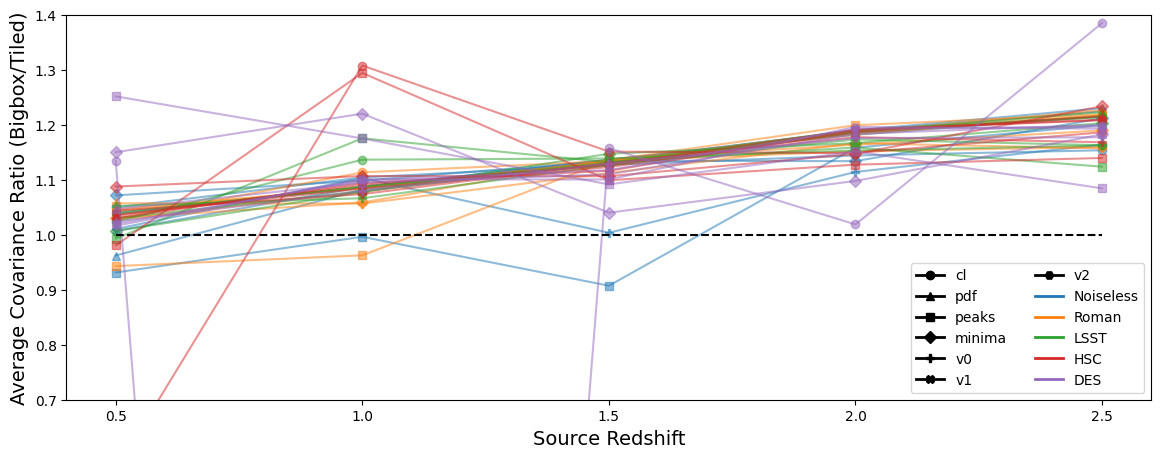
\includegraphics[width=\textwidth]{figures/results/avg_cov_ratio_ngal.png}
    \caption[Average BIGBOX/TILED Ratio of Covariance for multiple noise levels]{Average ratio of covariance matrices of statistical measures between the BIGBOX and TILED simulations for different shape noise levels (see Table~\ref{tab:survey_comparison}). The increasing trend indicates does not affected by the noise level.}
    \label{fig:avg_noise_cov}
    \vspace{2cm}
    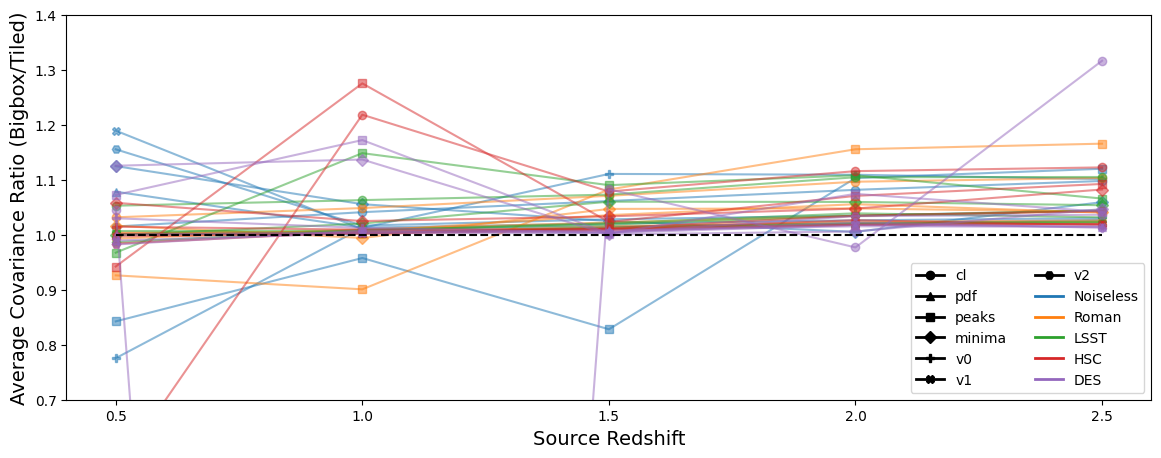
\includegraphics[width=\textwidth]{figures/results/avg_corr_ratio_ngal.png}
    \caption[Average BIGBOX/TILED Ratio of Correlation for multiple noise levels]{Same as Figure~\ref{fig:avg_noise_cov}, but for the correlation matrices. The off-diagonal elements compared to the diagonal elements do not show a clear trend with noise levels.}
    \label{fig:avg_noise_corr}
\end{figure}

\begin{figure}[p]
    \centering
    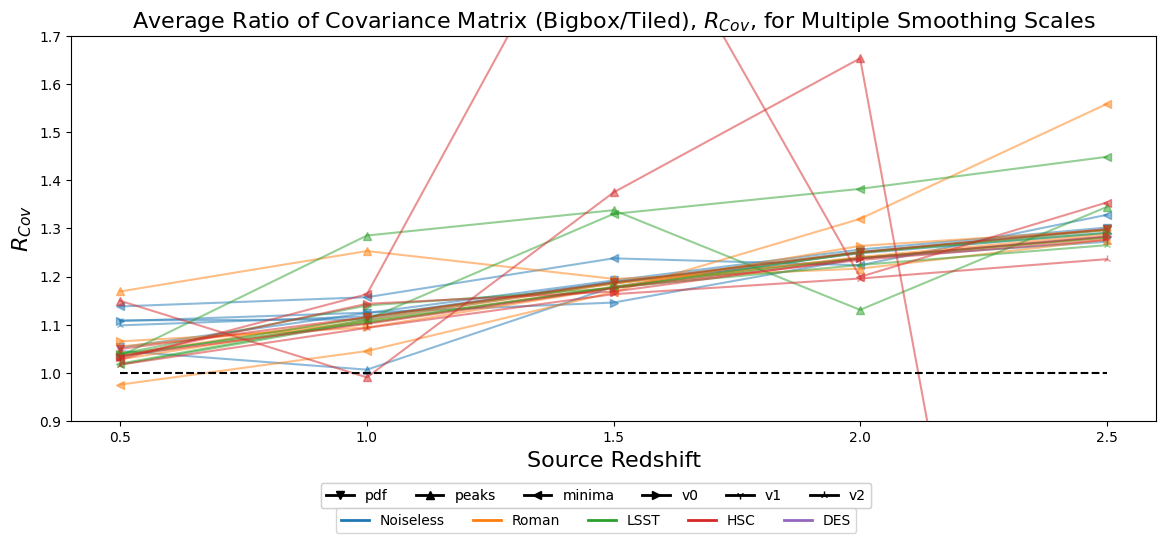
\includegraphics[width=\textwidth]{figures/results/avg_cov_ratio_sl.png}
    \caption[Average BIGBOX/TILED Ratio of Covariance for multiple smoothing scales]{Average ratio of covariance matrices of statistical measures between the BIGBOX and TILED simulations for different smoothing scales. Larger smoothing scales lead to increased discrepancies in covariance estimates due to the loss of small-scale information.}
    \label{fig:avg_sl_cov}
    \vspace{2cm}
    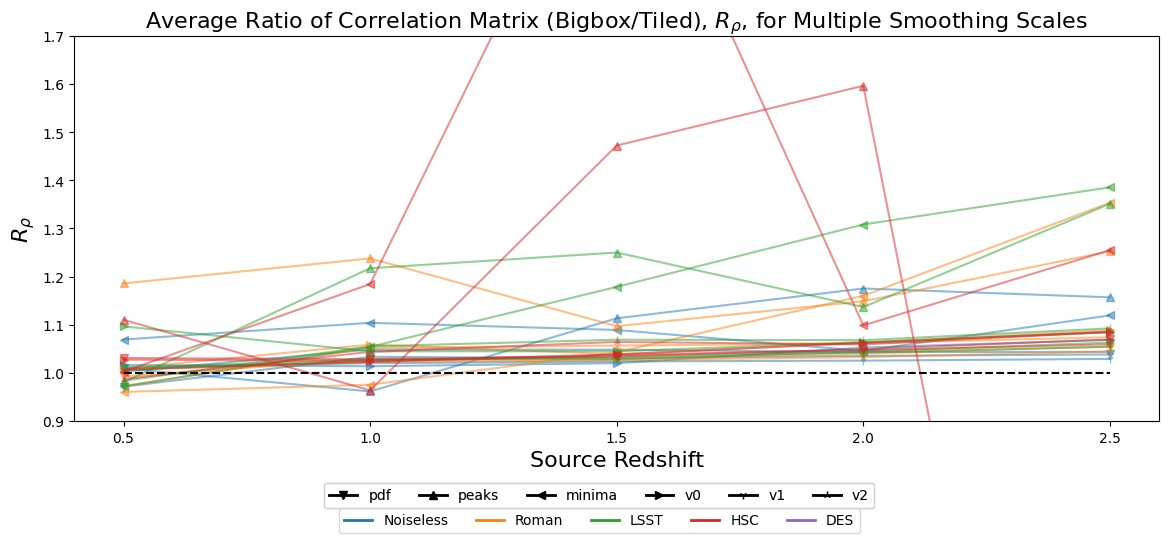
\includegraphics[width=\textwidth]{figures/results/avg_corr_ratio_sl.png}
    \caption[Average BIGBOX/TILED Ratio of Correlation for multiple smoothing scales]{Same as Figure~\ref{fig:avg_sl_cov}, but for the correlation matrices. The instability at larger smoothing scales reflects the challenges in capturing correlations at reduced resolutions.}
    \label{fig:avg_sl_corr}
\end{figure}

Figures~\ref{fig:cl_noise} and~\ref{fig:ng_noise} demonstrate how the ratios of covariance matrices for the angular power spectrum and the non-correlation statistics change with different shape noise levels. The results indicate that the angular power spectrum and minima are particularly sensitive to the shape noise level, exhibiting significant variations in their covariance matrices. In contrast, other non-correlation statistics remain more robust against changes in the shape noise level, maintaining relatively stable off-diagonal elements in their covariance matrices.

\begin{figure}[p]
    \centering
    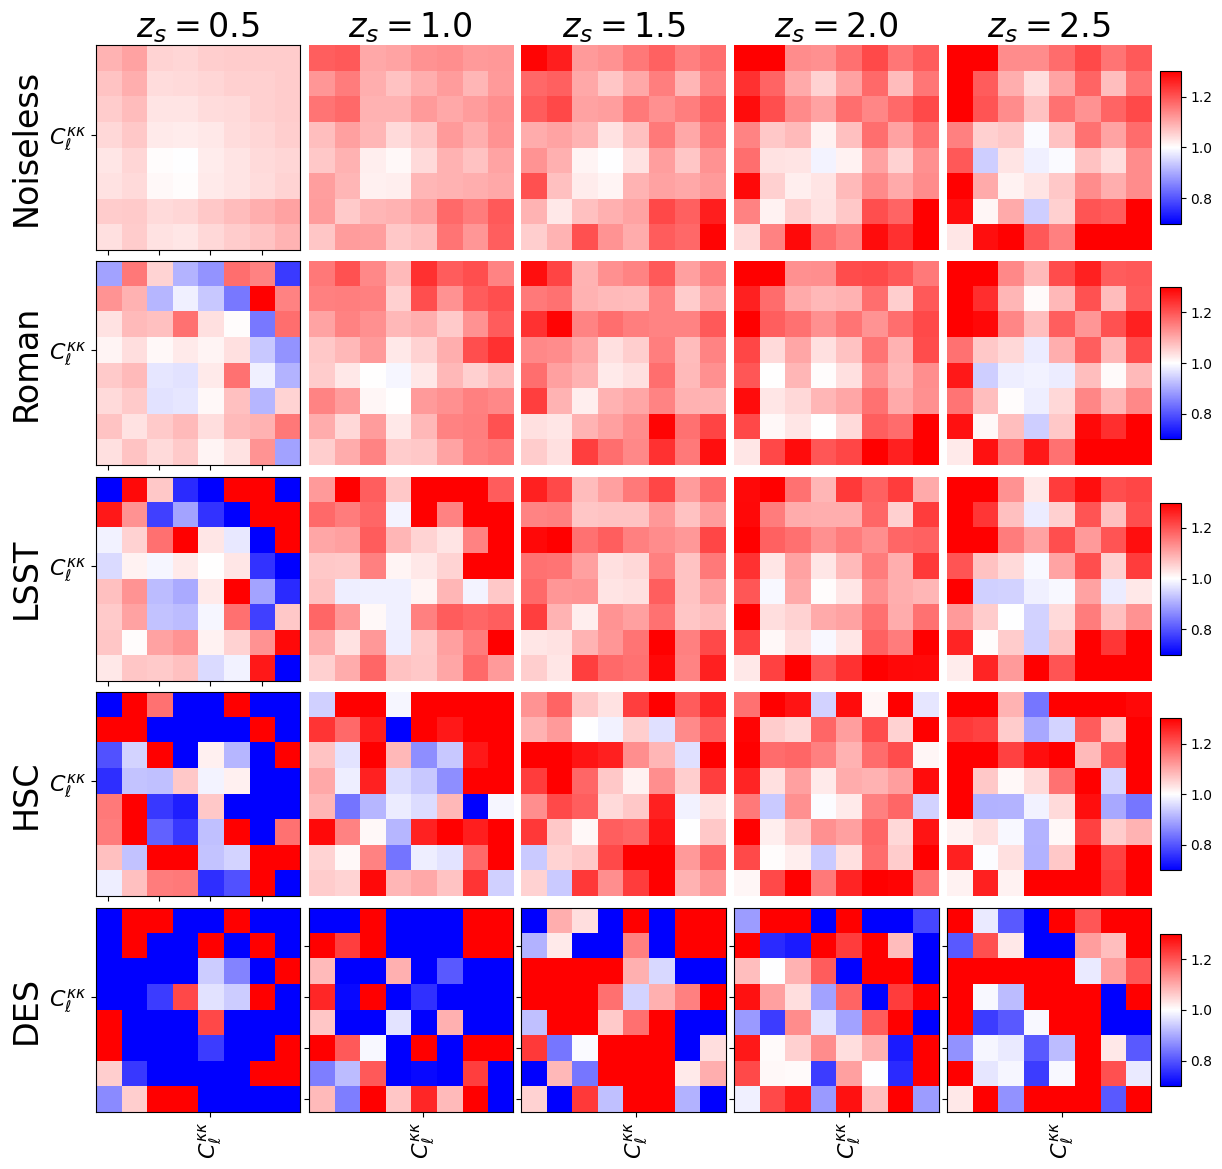
\includegraphics[width=0.6\textwidth]{figures/results/correlation_cov_noise.png}
    \caption[BIGBOX/TILED Ratio of Covariance Matricies for multiple noise levels: $C^{\kappa\kappa}_{\ell}$]{Ratio of covariance matrices of the angular power spectrum ($C^{\kappa\kappa}_{\ell}$) between the BIGBOX and TILED simulations for different shape noise levels (see Table~\ref{tab:survey_comparison}). The sensitivity of the power spectrum to noise is evident from the fluctuating covariance ratios with higher noise levels.}
    \label{fig:cl_noise}
    \vspace{0.5cm}
    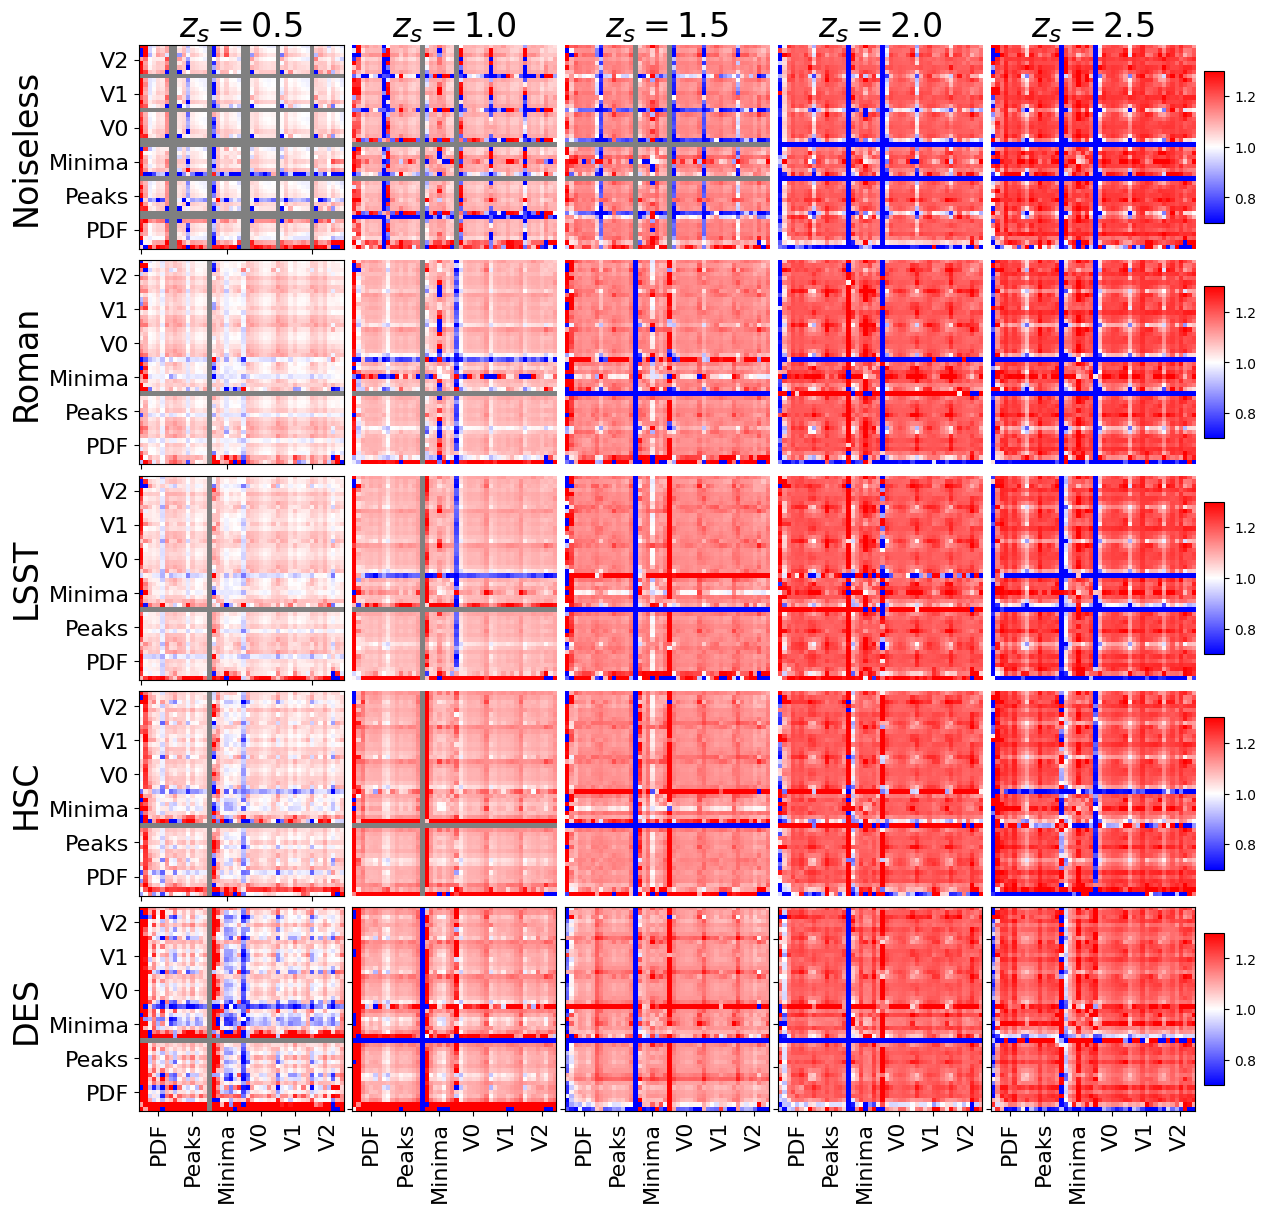
\includegraphics[width=0.8\textwidth]{figures/results/nongaussian_cov_noise.png}
    \caption[BIGBOX/TILED Ratio of Covariance Matricies for multiple noise levels: Non-Gaussian Statistics]{Same as Figure~\ref{fig:cl_noise}, but for the non-Gaussian statistical measures. The robustness of these measures against noise variations is reflected in the relatively stable covariance ratios.}
    \label{fig:ng_noise}
\end{figure}

\section{Effects of Smoothing Scale}
To evaluate the impact of smoothing on the statistical measures, we have applied four different smoothing scales to the simulations. Smoothing affects the resolution of the convergence maps and can influence the detection of small-scale structures.

Figures~\ref{fig:avg_sl_cov} and~\ref{fig:avg_sl_corr} show how the average ratios of covariance matrices and correlation matrices change with varying smoothing scales. The ratios become more unstable due to the smoothing effect washing out small-scale structures.

Figure~\ref{fig:ng_smoothing} illustrates the effects of smoothing scale on non-Correlation statistical measures. As the smoothing scale increases, the finer structures in the convergence maps are blurred, leading to changes in the statistical properties. The blank bins that previously contained little or no signal begin to be filled due to the spread of signals from neighboring bins, while the overall signal intensity is redistributed.

\begin{figure}[ht]
    \centering
    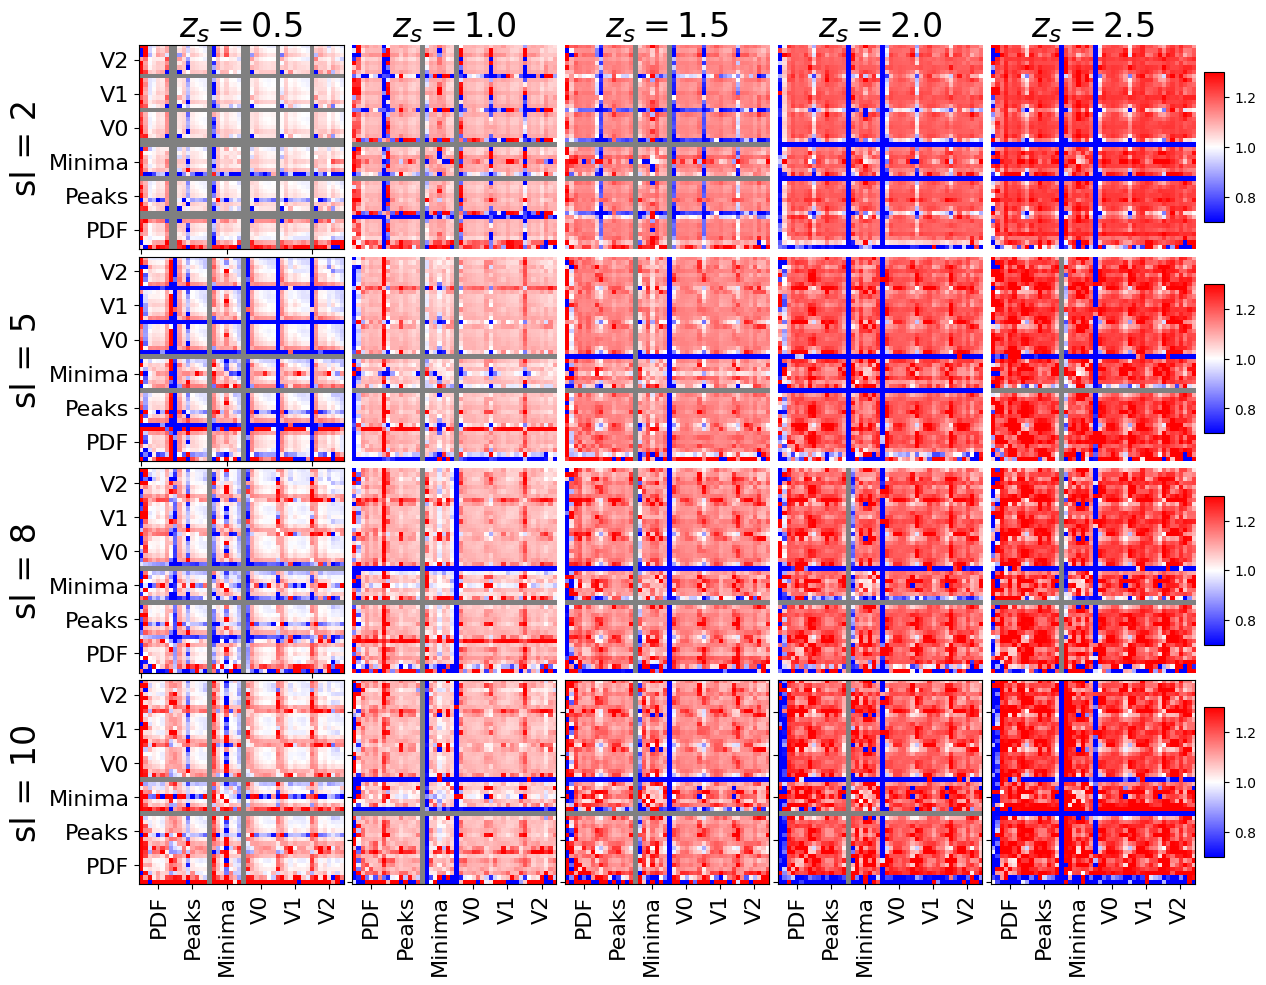
\includegraphics[width=0.8\textwidth]{figures/results/nongaussian_cov_sl.png}
    \caption[BIGBOX/TILED Ratio of Covariance Matricies for multiple smoothing scales: Non-Gaussian Statistics]{Same as Figure~\ref{fig:ng_noise}, but showing the impact of different smoothing scales on the covariance matrices of non-Gaussian statistical measures. The results emphasize how increased smoothing affects the detection and characterization of small-scale features.}
    \label{fig:ng_smoothing}
\end{figure}

\section{Source of Systematics}
In this section, we will discuss the possible sources of systematics that could affect the covariance matrix. 

\subsection{Box Replication Effect}\label{sec:boxreplication}
The box replication effect arises from replication of the simulation box in order to increase the volume of the simulation. In our setup, patches around special directions suffer the most from the box replication effect. To roughly assess the effect, we can compare the covariance matrices made from the patches of those directions and the rest of the patches.

Here, we defined the directions where are suspected to be affected by the box replication effect by the following criteria:
\begin{itemize}
    \item data points around equator: $ \left| \theta_i - \frac{\pi}{2} \right| \leq R_{\text{patch}} $
    \item data points around the edges of octant: $ \left| \phi_i - \frac{k\pi}{2} \right| \leq R_{\text{patch}} $ for $k=0,1,2,3$
\end{itemize}
where $(\theta_i, \phi_i)$ denotes the center of the patch $i$, and $R_{\text{patch}} = 5\sqrt{2}\, \mathrm{\deg}$ is the half diagonal length of the patch. 

We found that the patches including the point $(\theta_i, \phi_i) = (\pi/2, 0)$ have a signnificantly variated mean and variance, even comapared to the rest of suspects. Therefore, we simply discarded this point as it will bias the result. 

Finally, we obtain $70$ patches from each realization, and $1400$ patches for TILED simulations and $770$ patches for BIGBOX simulations in total.

Figure~\ref{fig:boxreplication_cov} and Figure~\ref{fig:boxreplication_corr} show the average ratios of the covariance matrices and correlation matrices between BIGBOX and TILED simulations. Regardless the noisy behavior of bispectrum, the ratio are much closer to unity for the suspected patches. This implies that the box replication effect is significantly enhance the covariance matrix.

\begin{figure}[ht]
    \centering
    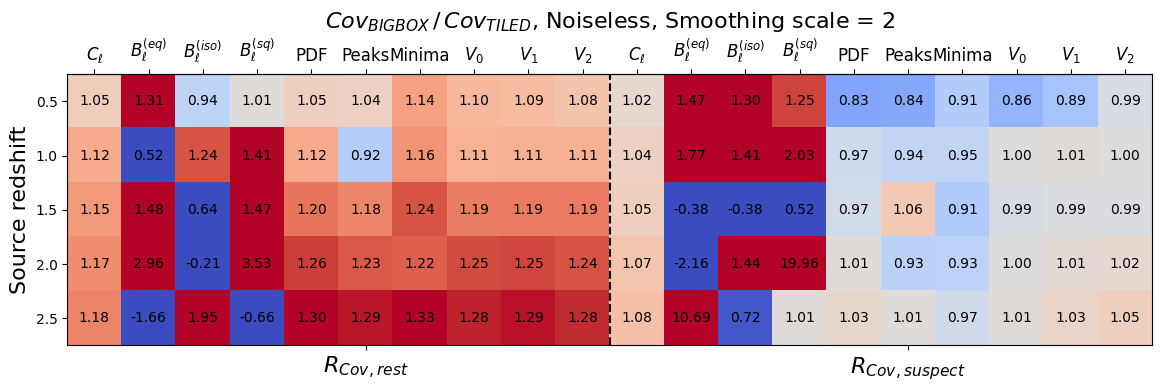
\includegraphics[width=\textwidth]{figures/BR_ratio_cov.png}
    \caption{The BIGBOX / TILED ratios of covariance matrices, for the case of the patches around special directions and the rest of the patches. }
    \label{fig:boxreplication_cov}
    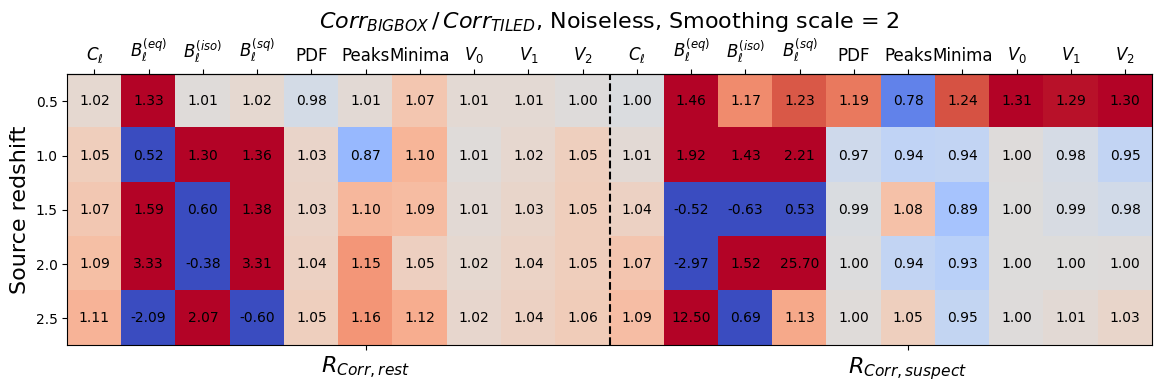
\includegraphics[width=\textwidth]{figures/BR_ratio_corr.png}
    \caption{The same as Figure~\ref{fig:boxreplication_cov}, but for correlation matrices.}
    \label{fig:boxreplication_corr}
\end{figure}

Figure~\ref{fig:boxreplication_ell} and~\ref{fig:boxreplication_nu} show the comparison of the ratios of mean and variance of each Statistics. Clearly, the suspected patches have biased mean values. The variance ratios are closer to unity, which means that the variance of the suspected patches is larger than the rest of the patches.

\begin{figure}[p]
    \centering
    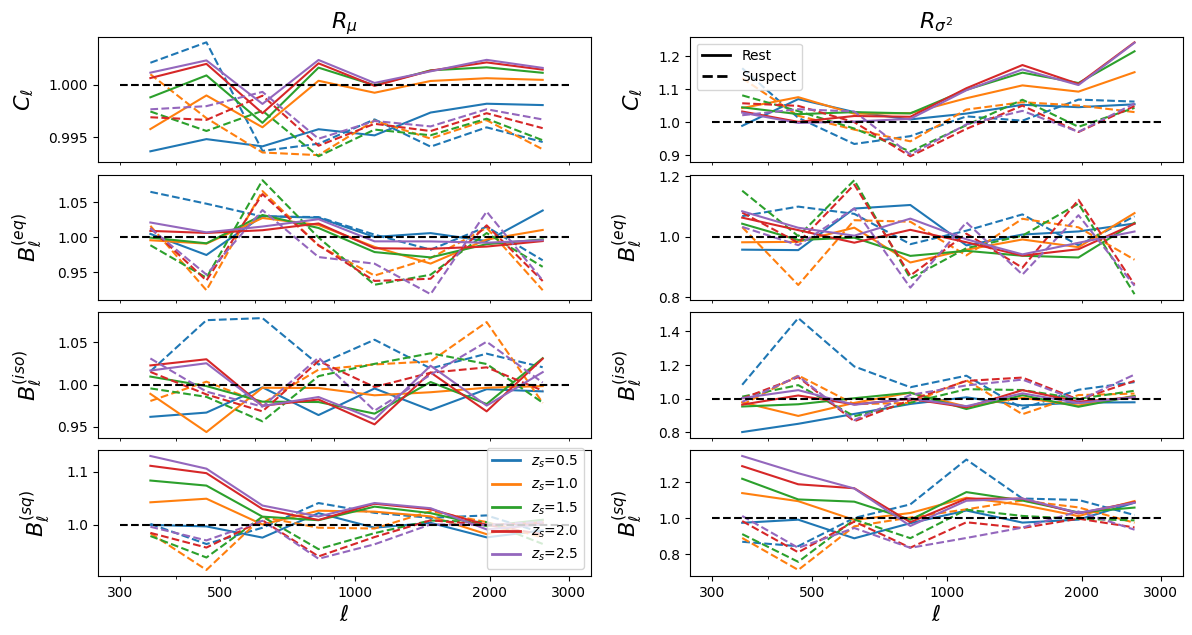
\includegraphics[width=0.9\textwidth]{figures/BR/BR_ratio_ell.png}
    \caption{The ratios of mean and variance of power spectrum and bispectrum between the patches around special directions and the rest of the patches. The mean of suspected patches are biased and the variance is larger.}
    \label{fig:boxreplication_ell}
    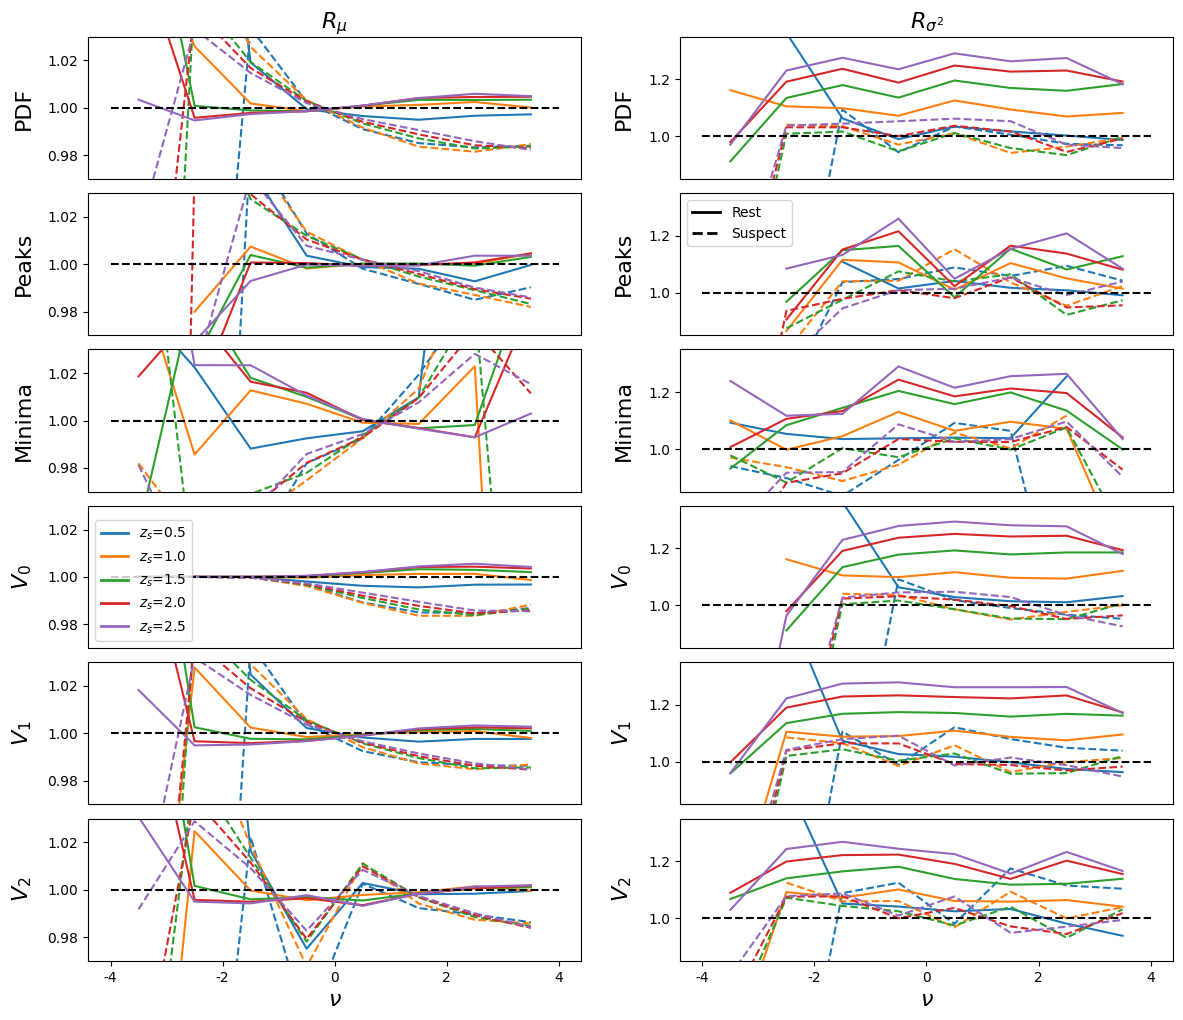
\includegraphics[width=0.9\textwidth]{figures/BR/BR_ratio_nu.png}
    \caption{The same as Figure~\ref{fig:boxreplication_ell}, but for PDF, peak/minima counts and Minkowski functionals. The suspected patches tend to have more extreme values and larger variance.}
    \label{fig:boxreplication_nu}
\end{figure}

\section{flat-sky vs. full-sky}
The flat-sky approximation is a good approximation for small patches on the sky. However, the flat-sky approximation breaks down for large patches. In this section, we conduct a test for angular power spectrum, PDF, and peak/minima counts to see how the flat-sky approximation affects the statistics.